\documentclass[11pt,a4paper]{book}
\usepackage[brazilian]{babel}
\usepackage[utf8]{inputenc}
\usepackage[T1]{fontenc}
\usepackage[inline]{enumitem}
\usepackage{xcolor}
\usepackage{listings}
\usepackage{graphicx}
\usepackage{multicol}
\usepackage{amsmath}

\definecolor{mGreen}{rgb}{0,0.6,0}
\definecolor{mGray}{rgb}{0.5,0.5,0.5}
\definecolor{mPurple}{rgb}{0.58,0,0.82}
\definecolor{backgroundColour}{rgb}{0.95,0.95,0.92}

\lstdefinestyle{CStyle}{
    backgroundcolor=\color{backgroundColour},   
    commentstyle=\color{mGreen},
    keywordstyle=\textbf{\color{black}},
    numberstyle=\tiny\color{mGray},
    stringstyle=\color{mPurple},
    basicstyle=\footnotesize,
    breakatwhitespace=false,         
    breaklines=true,                 
    captionpos=b,                    
    keepspaces=true,                 
    numbers=left,                    
    numbersep=5pt,                  
    showspaces=false,                
    showstringspaces=false,
    showtabs=false,                  
    tabsize=2,
    frame=single,
    escapeinside={(*}{*)},
    language=C
}

\makeatletter
% This command ignores the optional argument for itemize and enumerate lists
\newcommand{\inlineitem}[1][]{%
\ifnum\enit@type=\tw@
    {\descriptionlabel{#1}}
  \hspace{\labelsep}
\else
  \ifnum\enit@type=\z@
       \refstepcounter{\@listctr}\fi
    \quad\@itemlabel\hspace{\labelsep}
\fi}
\makeatother

\newcommand{\onestaritem}{\refstepcounter{enumi}\item[$*$\theenumi.]}
\newcommand{\twostaritem}{\refstepcounter{enumi}\item[$**$\theenumi.]}

\title{Lista 4: Fundamentos Estatísticos para Ciência dos Dados}
\author{Ricardo Pagoto Marinho}

\begin{document}
\maketitle
	\begin{enumerate}
		\item
			\begin{itemize}
				\item O valor de \textit{k} em que $P(X=k)$ é máxima é 3, com uma probabilidade de aproximadamente 0.25.
				\item Visualmente, a faixa [0,6] é a na qual a probabilidade se aproxima mais a 1.
				\item O entorno do valor n$\theta$ é o mais alto, já que no valor máximo de probabilidade é em 3.
				\item pbinom(6,20,0.15)-pbinom(0-0.01,20,0.15)
				
				0.9780649
				
				Como esperado, o valor é próximo a 1 no intervalo [0,6].
				A função pbinom faz o intervalo aberto com o valor passado, ou seja, (5,8].
				Para corrigir, isso, subtrai-se 0.01.
				\item qbinom(0.95,20,0.15)
				
				[1] 6
				
				\item pbinom(6,20,0.15)

				[1] 0.9780649
				
				\item
				Sim, 98\% dos números foram menores ou iguais a 6.
				
				\item dx<-dbinom(c(0:6),20,0.15)
				
				dx
				
				0.03875953 0.13679835 0.22933840 0.24282890 0.18212167 0.10284518 0.04537287
				
				sum(x==0)

				4
				
				sum(x==1)
				
				14
				
				sum(x==2)
				
				23
				
				sum(x==3)
				
				27
				
				sum(x==4)
				
				16
				
				sum(x==5)
				
				11
				
				sum(x==6)
				
				3
				
				Sim, os valores das probabilidades e das frequências relativas são parecidas.
			\end{itemize}
		\item
			\begin{itemize}
				\item
					\begin{figure}[t]
						\centering
						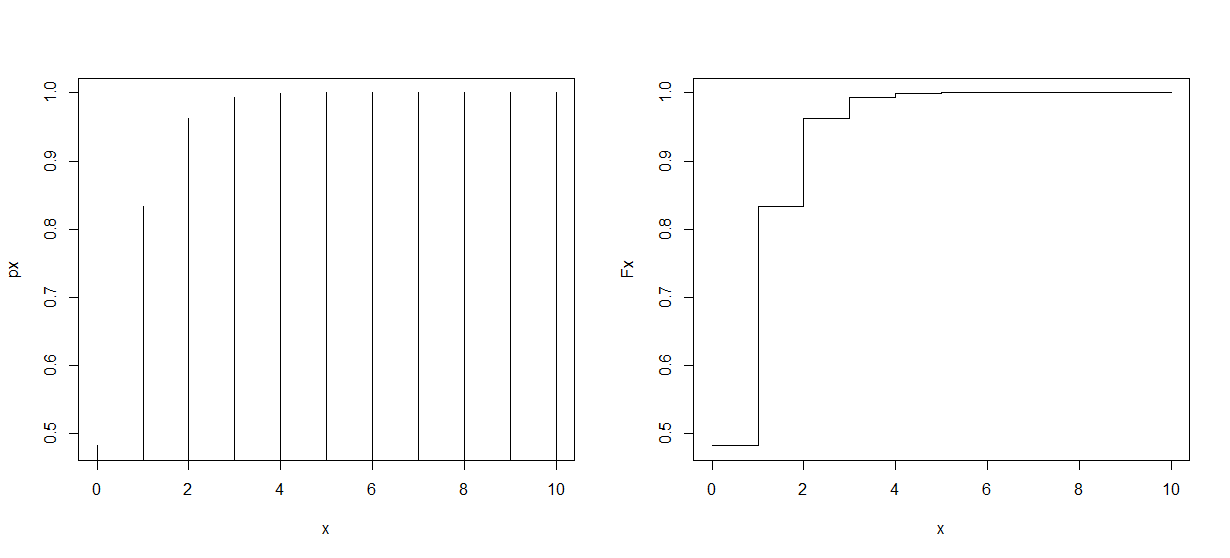
\includegraphics[height=5cm]{pois1.png}
						\caption{Distribuição de Poisson com $\lambda = 0.73$}
					\end{figure}
					\begin{figure}[t]
						\centering
						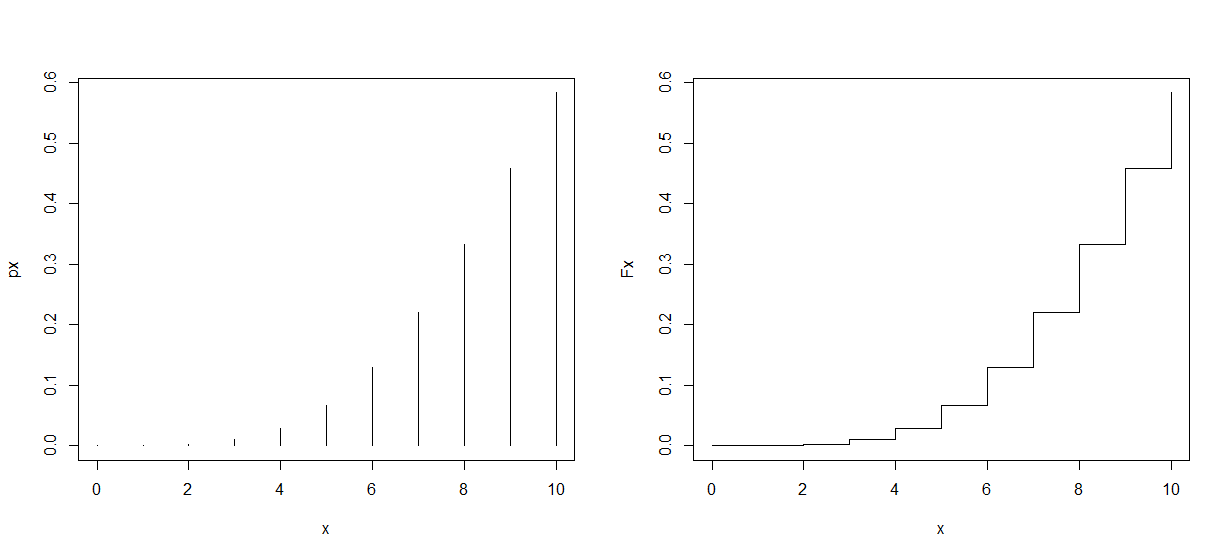
\includegraphics[height=5cm]{pois2.png}
						\caption{Distribuição de Poisson com $\lambda = 10$}
					\end{figure}
				\item
					Para $\lambda = 10$, o valor de $E(X)$ é próximo ao $P(X=k)$ máximo, porém para $\lambda = 0.73$ isso não ocorre.
				\item
					$\lambda = 0.73$: [1,10].
					
					$\lambda = 10$: [6,10].
				\item
					ppois(10,0.73)-ppois(1-0.01,0.73)

					[1] 0.518091
					
					ppois(10,10)-ppois(6-0.01,10)

					[1] 0.5159538
					
				\item
					rpois(200,0.73)
  
  					2 1 1 0 1 1 0 0 3 3 1 0 0 0 1 2 1 0 1 0 1 0 0 0 0 1 0 0 0 0 0 1 1 0 1 0 3 0 2 2 0 2 1 0 0 1 2 0 1 0 0 1 1 2 1 0 1 0 1 0 0 0 0 2 0 2 1 1 3 0 0 1 1 2 0 0 0 1 0 1 1 0 0 0 0 2 0 0 1 0 1 1 0 1 1 1 0 0 1 1 1 0 2 0 2 3 1 1 0 1 0 0 1 0 0 0 0 0 0 1 0 0 1 1 0 0 2 0 1 0 0 1 1 1 0 0 0 0 1 1 0 0 1 1 0 1 1 0 1 2 2 1 2 0 1 0 0 1 1 1 0 0 0 1 0 2 2 0 0 2 1 1 1 0 1 1 0 0 1 0 0 0 0 1 0 0 4 0 0 1 0 0 1 0 0 2 1 1 1 1
  					
  					rpois(200,10)
  
  					16 11  9 10  8  6 13  6 11  7  6 12 12 11 14 11  9 14 12 9 3 10 7 14 11 8 12 8 8 16 5 10 9 9 14 13 17 10 6 11 6 11 14 4 10 7 12 10 9 7 11 13 14 21 13  8  5 10 13  8  8  9  1 12  7 11 12  6  8  7  9 11 10  9  8  9  8 15 14  8 10 12  6 17 13 13 12 14 14 13 18  9 15 12 13 11 8  7  5 10 13 15  7 11 10 10 16  8  7 12 12 13  7 13 12 10  8  8 12 11 7 11 11  9 12  4  5 15  8  6  9 10  6 12  9 11  7  7 10 11  4 13  8 21 8  7 13  3 10 11 10 11 13  8 14  9  7 14  8 10  3  7  9  7 12  9 11  8 12  9  8  7 13  9 11  4 15 11  8 14  9  7 13 11 17  9 11  7  9 11  6 10 13 14  6 10  9  7 11  8]
  					
  				\item
  					dx<-dpois(c(0:6),0.73)

					dx

					0.4819089901 0.3517935628 0.1284046504 0.0312451316 0.0057022365 0.0008325265 0.0001012907
					
					sum(x==0)/200
					
					[1] 0.525
					
					sum(x==1)/200

					[1] 0.27

					sum(x==2)/200

					[1] 0.16
					
					sum(x==3)/200

					0.04
				
					sum(x==4)/200
					
					[1] 0.005

					sum(x==5)/200

					[1] 0
	
					sum(x==6)/200
		
					[1] 0
					
					dx
					
					4.539993e-05 4.539993e-04 2.269996e-03 7.566655e-03 1.891664e-02 3.783327e-02 6.305546e-02
					
					sum(x==0)/200
					
					[1] 0

					sum(x==1)/200

					[1] 0
	
					sum(x==2)/200
					
					[1] 0
				
					sum(x==3)/200
					
					[1] 0.01

					sum(x==4)/200
					
					[1] 0.01
					
					sum(x==5)/200

					[1] 0.035
			
					sum(x==6)/200
					
					[1] 0.085
			\end{itemize}
		\item
			\begin{itemize}
				\item
					\begin{figure}[t]
						\centering
						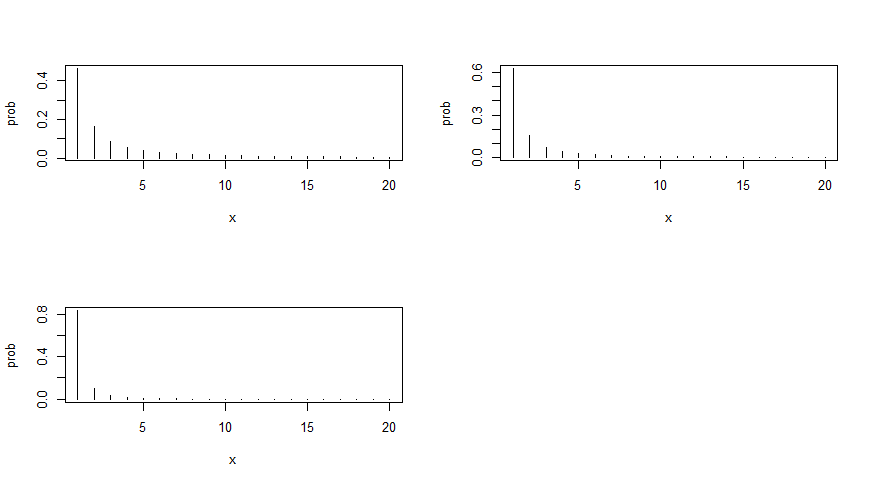
\includegraphics[height=6cm]{3-1.png}
						\caption{P(X=k), $\alpha=$1/2,1,2}
					\end{figure}
					\begin{figure}[t]
						\centering
						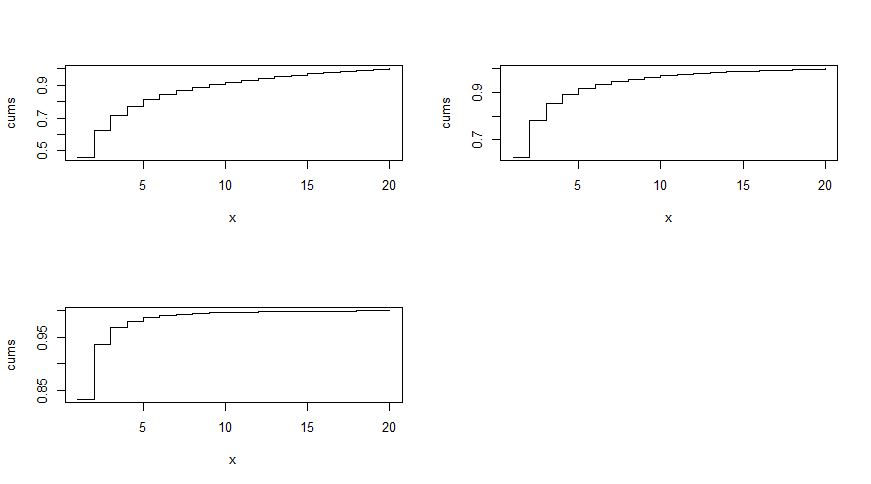
\includegraphics[height=6cm]{csum.png}
						\caption{F(X=k),$\alpha=$1/2,1,2}
					\end{figure}
				\item
				rzipf(400,1/2,1/2.262)
				
				2  1  1  5  4  2  2  1  1  5  1  1  1  2  1  1 4  1  2  5  1  1  1  4  2  4  2  4  1  1  2 12 4  6  3  5  4  2  1  1  1  1  1  2  5  1  1  1 6  1  2  1 28 14  4  3  2  1  2  2  1  1  4  1 1  1  1  3  1 14  6  1  9  1  4  1  1  4  2  2 3  4  1  2  2  4  1  5  1  1  4  4  1  1  9 14 1  1  1  1  4  2  1 24  4  4  1  1  3  1  1  2 2  1  2  1  1 28 28  3  5 13 10  4  2  7 23  1 11  1  3  1  1  1  1  1  3  1  3  2  5  1  1 23 1  1  1  2  7  3  9  1 14  1  4  1  2  1  4  4 20 20  4  2  4  2  5  6  1 30  1  1  2 17  1  5 6  2  1  2  1  2  2  2  2 16  1  1  1  3  1  1 1  1  1  1  1  2  2  3  3  1  1  1  1  2 25  2 2  3  1 11 24  5 31  4  4  1  2  3  1  7  2  3 17  5  1  1  7  2  1  2  5  1  1  1  1 13  1  1 1  1  1  4  1  1 24 19  2  1  1  1  1  1 15 23 14  1  1 16  1  4  4  2  1  2  1  7  2  2  1  5 20  1  2  3  1 21  1  1  1  2  1 10  1  1 12  1 2  1  8  1  8  4  1  1  1  1  1  1  1  2  8  1 3  2  3  1  3  1  1  6  1 13  1  1 20  1  1  7 1  8  4  1 12  2  1  2  3 23  2  2  3  1  1 10 1  1  1  2  1  5  3 27  2  5  1  5  5  1  1  8 5  1  1  1  1  6  1 14  1 12  3  1  1 30  1  1 4  1  2  3  1  2  1  2  1  4  1  3  1  1  2  1 1  6  2  1 26  2  2  2  1  1  2  1  2  2  1  2
			\end{itemize}
	\end{enumerate}
\end{document}